\documentclass[12pt]{article}

\usepackage{epsfig}
\usepackage{amsmath}

\begin{document}
\noindent
Luke Palmer                 \\
8/31/2004                   \\
Writeup of CAPA Problem 1-4

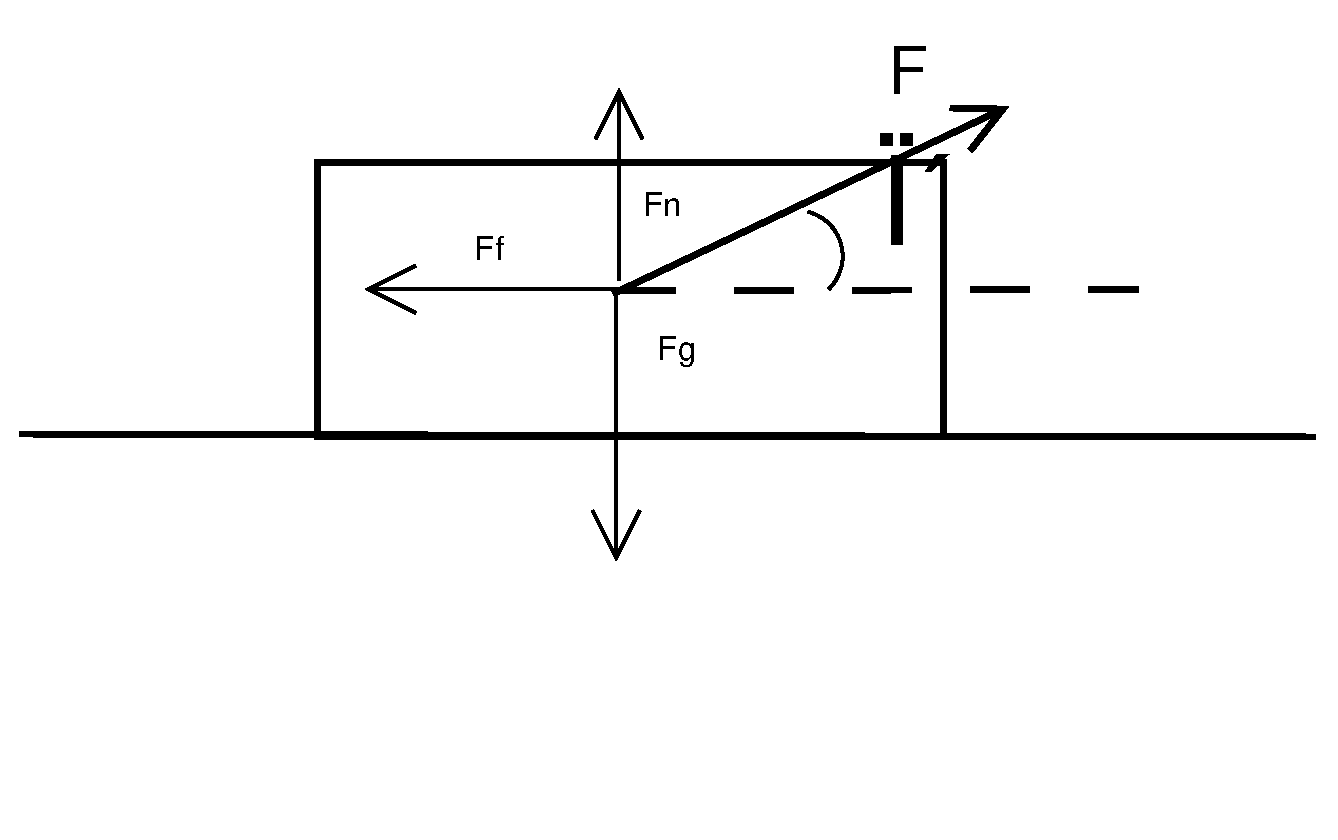
\epsfig{file=freebody.eps,height=3in}

The essence of this problem is to compute the force exerted by friction.  For
that we need the normal force, which is just the force gravity is exerting
on the box minus the vertical component of the pulling force.  Assuming $g$ 
is negative:

\[
    F_n = -g M - F \sin{\theta}
\]

From there it is trivial to find the force of friction:

\[
    F_f = \mu F_n
\]

So the total rightward force, accounting for friction is:

\[
    F_t = F \cos{\theta} - F_f
\]

And it follows that the speed after time $t$ is:

\begin{align*}
    v &= t \frac{F_t}{M} \\
      &= t \frac{F \cos{\theta} - \mu (-g M - F \sin{\theta})}{M}
\end{align*}


\end{document}
